%****************************************************************************
%** Copyright 2002 by Lukas Ruf, ruf@topsy.net
%** Information is provided under the terms of the
%** GNU Free Documentation License http://www.gnu.org/copyleft/fdl.html
%** Fairness: Cite the source of information, visit http://www.topsy.net
%****************************************************************************
%****************************************************************************
%** Last Modification: 2005-07-11 1600
%** 2005-07-11	Bernhard Tellenbach
%**							This is an addapted version of the Introduction.tex file
%**							Added table example (footnotes,multicolumn)
%**							Examples for different text sizes
%**							Updated eps file inclusion example for use with graphicx pkt. 
%****************************************************************************

\chapter{\label{chapter2}Title}
In \ref{introduction} we start with our introduction to the problem that we 
are going to address.  Since we do not want to waste the readers time we 
go and show the essential issues of latex in section
\ref{chapter2:essentials}.

\section{\label{chapter2:essentials}Essentials}

Well this section can be further subdivided into subsection.  We present 
this in subsection \ref{chapter2:essentials:subsections}.

\subsection{\label{chapter2:essentials:subsections}Subsections}

\paragraph{\label{introduction:essentials:subsections:paragraph}Paragraphs}
can be specially referenced as well.

Of further importance is the understanding of the following environments:

%*** itemized lists
\begin{itemize}
\item This shows an itemized bullet list
  \begin{itemize}
  \item Which can be used for several levels\ldots
  \end{itemize}
\end{itemize}

%*** enumerated lists
\begin{enumerate}
\item The same applies to enumerated lists.
\end{enumerate}

\begin{figure}[!hbt]
  \begin{center}
		 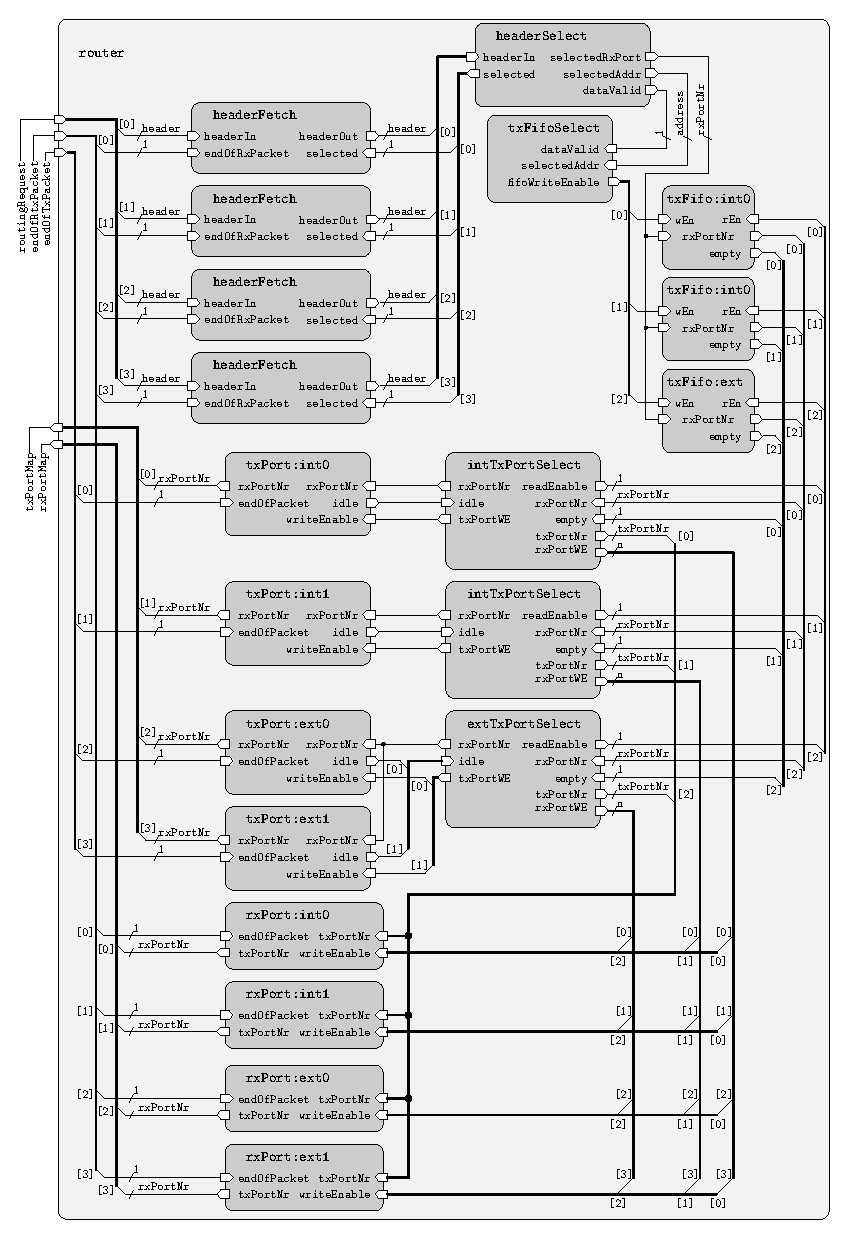
\includegraphics[width=\textwidth]{router.eps}
  \caption{This is a figure to be printed in a float}
  \label{router.eps}
  \end{center}
\end{figure}
By figure \ref{router.eps}, we show some funny figures.


Table with caption and footnotes below the table.

\begin{table}[htbp]
\begin{center}\begin{minipage}{\textwidth}
\begin{tabular}{| c | p{130pt} | l |}
\hline
Column 1 & Column 2 \newline (additional line) & Column 3 \\
\hline
C1,R2 & C2,R2 & C2,R3 \\
\hline
C1,R3	& \multicolumn{2}{| c |}{C2\&C3,R3} \\
\hline
C1,R4 & C2,R4\footnote{Footnote to table~\ref{tab:table1}} & C3,R4\\
\hline
\end{tabular}
\end{minipage}
\caption{Table 1}
\label{tab:table1}
\end{center}
\end{table}

Examples of different text sizes:

\small Small \\
\scriptsize Script size \\
\normalsize Normal \\
\large Large \\
\huge Huge \\
\normalsize

\CHECK
If we reference to another document, we cite the document \cite{bib:relevantwork}.

%** landscape
\NEW
\begin{landscape}
Of some interest is also the landscape environment:
\end{landscape}

\verbatiminput{filename.txt}
Even though we don't think full listings are useful in documents,
you can easily insert complete files by the verbatiminput{}-command.

